% edge_label_derivation.tex
% K5 v pentagonálnom rozmiestnení. Tour = vonkajší päťuholník (y=1),
% diagonály = non-tour (y=0). Len legenda, bez inline štítkov.
% Použitie: \resizebox{0.55\textwidth}{!}{% edge_label_derivation.tex
% K5 v pentagonálnom rozmiestnení. Tour = vonkajší päťuholník (y=1),
% diagonály = non-tour (y=0). Len legenda, bez inline štítkov.
% Použitie: \resizebox{0.55\textwidth}{!}{% edge_label_derivation.tex
% K5 v pentagonálnom rozmiestnení. Tour = vonkajší päťuholník (y=1),
% diagonály = non-tour (y=0). Len legenda, bez inline štítkov.
% Použitie: \resizebox{0.55\textwidth}{!}{% edge_label_derivation.tex
% K5 v pentagonálnom rozmiestnení. Tour = vonkajší päťuholník (y=1),
% diagonály = non-tour (y=0). Len legenda, bez inline štítkov.
% Použitie: \resizebox{0.55\textwidth}{!}{\input{figures/tikz/edge_label_derivation}}
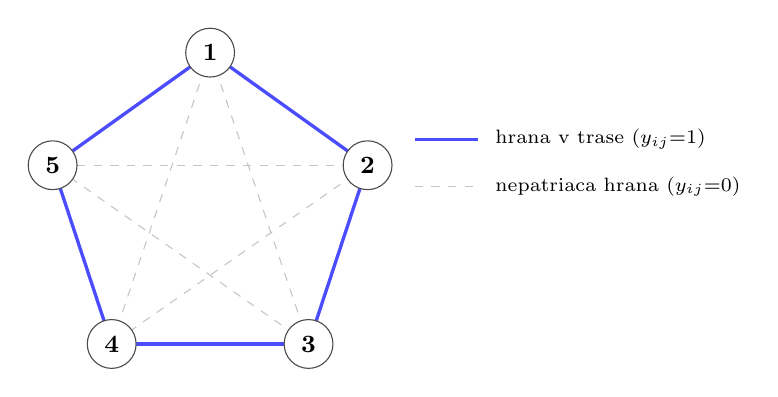
\begin{tikzpicture}[
    font=\small,
    vtx/.style={
        circle, draw=black!70, fill=white,
        minimum size=0.62cm, inner sep=1pt,
        font=\small\bfseries
    },
    touredge/.style={draw=blue!70, very thick},
    nonedge/.style={draw=gray!45, dashed, thin}
]

%% Vrcholy pravidelného päťuholníka r=2.1, stred=(2.60, 2.50)
\coordinate (v1) at (2.60, 4.60);
\coordinate (v2) at (4.60, 3.17);
\coordinate (v3) at (3.85, 0.90);
\coordinate (v4) at (1.35, 0.90);
\coordinate (v5) at (0.60, 3.17);

%% ── Diagonály (non-tour, y=0) ────────────────────────────────────
\draw[nonedge] (v1) -- (v3);
\draw[nonedge] (v1) -- (v4);
\draw[nonedge] (v2) -- (v4);
\draw[nonedge] (v2) -- (v5);
\draw[nonedge] (v3) -- (v5);

%% ── Vonkajší päťuholník (tour, y=1) ─────────────────────────────
\draw[touredge] (v1) -- (v2);
\draw[touredge] (v2) -- (v3);
\draw[touredge] (v3) -- (v4);
\draw[touredge] (v4) -- (v5);
\draw[touredge] (v5) -- (v1);

%% ── Vrcholy ──────────────────────────────────────────────────────
\node[vtx] at (v1) {1};
\node[vtx] at (v2) {2};
\node[vtx] at (v3) {3};
\node[vtx] at (v4) {4};
\node[vtx] at (v5) {5};

%% ── Legenda ──────────────────────────────────────────────────────
\draw[touredge] (5.20, 3.50) -- (6.00, 3.50);
\node[font=\scriptsize, anchor=west] at (6.10, 3.50)
    {hrana v trase (\(y_{ij}{=}1\))};
\draw[nonedge]  (5.20, 2.90) -- (6.00, 2.90);
\node[font=\scriptsize, anchor=west] at (6.10, 2.90)
    {nepatriaca hrana (\(y_{ij}{=}0\))};

\end{tikzpicture}}
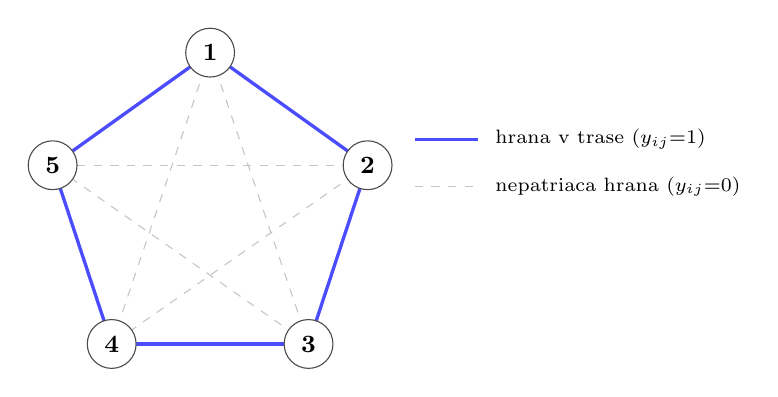
\begin{tikzpicture}[
    font=\small,
    vtx/.style={
        circle, draw=black!70, fill=white,
        minimum size=0.62cm, inner sep=1pt,
        font=\small\bfseries
    },
    touredge/.style={draw=blue!70, very thick},
    nonedge/.style={draw=gray!45, dashed, thin}
]

%% Vrcholy pravidelného päťuholníka r=2.1, stred=(2.60, 2.50)
\coordinate (v1) at (2.60, 4.60);
\coordinate (v2) at (4.60, 3.17);
\coordinate (v3) at (3.85, 0.90);
\coordinate (v4) at (1.35, 0.90);
\coordinate (v5) at (0.60, 3.17);

%% ── Diagonály (non-tour, y=0) ────────────────────────────────────
\draw[nonedge] (v1) -- (v3);
\draw[nonedge] (v1) -- (v4);
\draw[nonedge] (v2) -- (v4);
\draw[nonedge] (v2) -- (v5);
\draw[nonedge] (v3) -- (v5);

%% ── Vonkajší päťuholník (tour, y=1) ─────────────────────────────
\draw[touredge] (v1) -- (v2);
\draw[touredge] (v2) -- (v3);
\draw[touredge] (v3) -- (v4);
\draw[touredge] (v4) -- (v5);
\draw[touredge] (v5) -- (v1);

%% ── Vrcholy ──────────────────────────────────────────────────────
\node[vtx] at (v1) {1};
\node[vtx] at (v2) {2};
\node[vtx] at (v3) {3};
\node[vtx] at (v4) {4};
\node[vtx] at (v5) {5};

%% ── Legenda ──────────────────────────────────────────────────────
\draw[touredge] (5.20, 3.50) -- (6.00, 3.50);
\node[font=\scriptsize, anchor=west] at (6.10, 3.50)
    {hrana v trase (\(y_{ij}{=}1\))};
\draw[nonedge]  (5.20, 2.90) -- (6.00, 2.90);
\node[font=\scriptsize, anchor=west] at (6.10, 2.90)
    {nepatriaca hrana (\(y_{ij}{=}0\))};

\end{tikzpicture}}
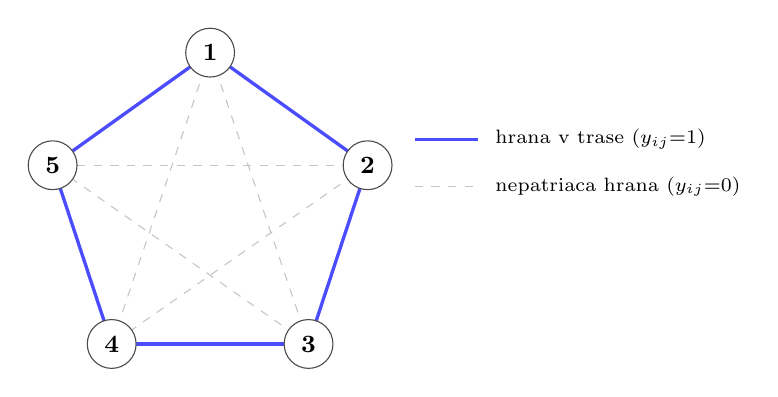
\begin{tikzpicture}[
    font=\small,
    vtx/.style={
        circle, draw=black!70, fill=white,
        minimum size=0.62cm, inner sep=1pt,
        font=\small\bfseries
    },
    touredge/.style={draw=blue!70, very thick},
    nonedge/.style={draw=gray!45, dashed, thin}
]

%% Vrcholy pravidelného päťuholníka r=2.1, stred=(2.60, 2.50)
\coordinate (v1) at (2.60, 4.60);
\coordinate (v2) at (4.60, 3.17);
\coordinate (v3) at (3.85, 0.90);
\coordinate (v4) at (1.35, 0.90);
\coordinate (v5) at (0.60, 3.17);

%% ── Diagonály (non-tour, y=0) ────────────────────────────────────
\draw[nonedge] (v1) -- (v3);
\draw[nonedge] (v1) -- (v4);
\draw[nonedge] (v2) -- (v4);
\draw[nonedge] (v2) -- (v5);
\draw[nonedge] (v3) -- (v5);

%% ── Vonkajší päťuholník (tour, y=1) ─────────────────────────────
\draw[touredge] (v1) -- (v2);
\draw[touredge] (v2) -- (v3);
\draw[touredge] (v3) -- (v4);
\draw[touredge] (v4) -- (v5);
\draw[touredge] (v5) -- (v1);

%% ── Vrcholy ──────────────────────────────────────────────────────
\node[vtx] at (v1) {1};
\node[vtx] at (v2) {2};
\node[vtx] at (v3) {3};
\node[vtx] at (v4) {4};
\node[vtx] at (v5) {5};

%% ── Legenda ──────────────────────────────────────────────────────
\draw[touredge] (5.20, 3.50) -- (6.00, 3.50);
\node[font=\scriptsize, anchor=west] at (6.10, 3.50)
    {hrana v trase (\(y_{ij}{=}1\))};
\draw[nonedge]  (5.20, 2.90) -- (6.00, 2.90);
\node[font=\scriptsize, anchor=west] at (6.10, 2.90)
    {nepatriaca hrana (\(y_{ij}{=}0\))};

\end{tikzpicture}}
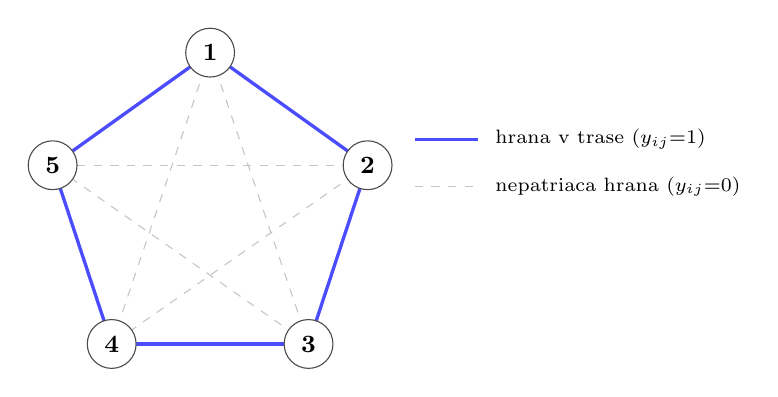
\begin{tikzpicture}[
    font=\small,
    vtx/.style={
        circle, draw=black!70, fill=white,
        minimum size=0.62cm, inner sep=1pt,
        font=\small\bfseries
    },
    touredge/.style={draw=blue!70, very thick},
    nonedge/.style={draw=gray!45, dashed, thin}
]

%% Vrcholy pravidelného päťuholníka r=2.1, stred=(2.60, 2.50)
\coordinate (v1) at (2.60, 4.60);
\coordinate (v2) at (4.60, 3.17);
\coordinate (v3) at (3.85, 0.90);
\coordinate (v4) at (1.35, 0.90);
\coordinate (v5) at (0.60, 3.17);

%% ── Diagonály (non-tour, y=0) ────────────────────────────────────
\draw[nonedge] (v1) -- (v3);
\draw[nonedge] (v1) -- (v4);
\draw[nonedge] (v2) -- (v4);
\draw[nonedge] (v2) -- (v5);
\draw[nonedge] (v3) -- (v5);

%% ── Vonkajší päťuholník (tour, y=1) ─────────────────────────────
\draw[touredge] (v1) -- (v2);
\draw[touredge] (v2) -- (v3);
\draw[touredge] (v3) -- (v4);
\draw[touredge] (v4) -- (v5);
\draw[touredge] (v5) -- (v1);

%% ── Vrcholy ──────────────────────────────────────────────────────
\node[vtx] at (v1) {1};
\node[vtx] at (v2) {2};
\node[vtx] at (v3) {3};
\node[vtx] at (v4) {4};
\node[vtx] at (v5) {5};

%% ── Legenda ──────────────────────────────────────────────────────
\draw[touredge] (5.20, 3.50) -- (6.00, 3.50);
\node[font=\scriptsize, anchor=west] at (6.10, 3.50)
    {hrana v trase (\(y_{ij}{=}1\))};
\draw[nonedge]  (5.20, 2.90) -- (6.00, 2.90);
\node[font=\scriptsize, anchor=west] at (6.10, 2.90)
    {nepatriaca hrana (\(y_{ij}{=}0\))};

\end{tikzpicture}